% !TEX root = thesis.tex
\documentclass[12pt,a4paper,titlepage,listof=totoc,bibliography=totoc,chapteratlists=0pt]{scrreprt}
\begin{filecontents*}{\jobname.xmpdata}
	\Keywords{PlanfredCRM, Kundenmanagement Tool}
	\Title{PlanfredCRM}
	\Author{Felix Arzt, Nico Obermair, Timo Mittermayr}
\end{filecontents*}

\setcounter{tocdepth}{3}

\usepackage[utf8]{inputenc}
\usepackage[T1]{fontenc}
\usepackage{amsmath}
\usepackage{amsfonts}
\usepackage{amssymb}
\usepackage[table]{xcolor}
\usepackage{graphicx}
\usepackage[left=3.50cm, right=2.00cm, top=2.00cm, bottom=2.00cm,foot=1cm]{geometry}
\usepackage[splitrule,hang,flushmargin,multiple,bottom]{footmisc}
\usepackage{lmodern, textcomp}
\usepackage{lmodern}
\usepackage{pdfpages}
\usepackage[ngerman]{babel}
\usepackage{multicol}
\usepackage{float}
\usepackage{array,tabularx,booktabs}
\usepackage{ragged2e}
\usepackage{lipsum}
\usepackage{wrapfig}

\newcolumntype{M}[1]{>{\centering\arraybackslash}m{#1}}

\usepackage{enumitem}
\newlist{compactitem}{itemize}{3}
\setlist[compactitem,1]{label=\textbullet, nosep,leftmargin=1.5em,labelwidth=*,align=left}
\setlist[compactitem,2]{label=--, nosep,leftmargin=1.5em,labelwidth=*,align=left}
\setlist[compactitem,3]{label=\textopenbullet, nosep,leftmargin=1.5em,labelwidth=*,align=left}
\newlist{compactenum}{enumerate}{3}
\setlist[compactenum,1]{label=\arabic*., nosep,leftmargin=1.5em,labelwidth=*,align=left}
\setlist[compactenum,2]{label=\alph*., nosep,leftmargin=1.5em,labelwidth=*,align=left}
\setlist[compactenum,3]{label=\roman*., nosep,leftmargin=1.5em,labelwidth=*,align=left}
\newlist{compactdesc}{description}{3}
\setlist[compactdesc]{leftmargin=1.5em,labelwidth=*,align=left}

\usepackage{microtype}

\usepackage[parfill]{parskip}

\definecolor{bluekeywords}{rgb}{0.13,0.13,1}
\definecolor{greencomments}{rgb}{0,0.5,0}
\definecolor{redstrings}{rgb}{0.9,0,0}
\definecolor{lightgray}{gray}{0.9}
\definecolor{lightblue}{rgb}{0.93,0.95,1.0}

\usepackage{listings}

\makeatletter
\lstdefinestyle{lststyle}{
	basicstyle=%
	\ttfamily
	\lst@ifdisplaystyle\scriptsize\fi
}
\makeatother

\renewcommand{\lstlistlistingname}{List of Listings}
% TODO: define other languages as needed
\lstset{language=Python,
numbers=left,               
numberstyle=\tiny,          
showspaces=false,
showtabs=false,
breaklines=true,
lineskip=-1pt,
tabsize=2,
showstringspaces=false,
breakatwhitespace=true,
escapeinside={(*@}{@*)},
commentstyle=\color{greencomments},
keywordstyle=\color{bluekeywords}\bfseries,
stringstyle=\color{redstrings},
style=lststyle,
xleftmargin=17pt,
         framexleftmargin=17pt,
         framexrightmargin=5pt,
         framexbottommargin=4pt
}
\lstset{
morekeywords={base,var,in,out,dynamic,from,where,select,orderby,function,\$,group,by,into,yield,async,await,@,None,self,as,elif,with}
}
\lstdefinelanguage{TypeScript}{
	keywords={typeof, new, true, false, catch, function, return, null, switch, var, if, in, while, do, else, case, break, void, number, string, boolean, module, \$, export, for, this},
	keywordstyle=\color{blue}\bfseries,
	ndkeywords={class, export, boolean, throw, implements, import, this},
	ndkeywordstyle=\color{darkgray}\bfseries,
	identifierstyle=\color{black},
	sensitive=false,
	comment=[l]{//},
	morecomment=[s]{/*}{*/},
	commentstyle=\color{purple}\ttfamily,
	stringstyle=\color{red}\ttfamily,
	morestring=[b]',
	morestring=[b]"
}
\usepackage{caption}
\DeclareCaptionFont{white}{\color{white}}
\DeclareCaptionFormat{listing}{\colorbox[cmyk]{0.43, 0.35, 0.35,0.01}{\parbox{\textwidth}{\hspace{10pt}#1#2#3}}}
\captionsetup[lstlisting]{format=listing,labelfont=white,textfont=white} 
\captionsetup[table]{justification=centering, singlelinecheck=false}

\usepackage{subcaption}

\usepackage{setspace}
\newcommand{\MSonehalfspacing}{%
	\setstretch{1.44}%  default
	\ifcase \@ptsize \relax % 10pt
	\setstretch {1.448}%
	\or % 11pt
	\setstretch {1.399}%
	\or % 12pt
	\setstretch {1.433}%
	\fi
}

\newcommand{\setauthor}[1]{\ohead[]{#1}}

\usepackage[automark]{scrlayer-scrpage}
\pagestyle{scrheadings}
\automark{chapter}
\renewcommand\sectionmark[1]{\markright{\MakeMarkcase {\thesection\hskip .5em\relax#1}}}
\rohead{\ifnum\expandafter\pdfstrcmp\botmark=0 \rightmark\else\leftmark{} --- \rightmark\fi}
\ihead[]{\headmark}
\chead[]{}
\ohead{}
\cfoot[]{}
\ofoot[\pagemark]{\pagemark}
\setheadsepline{.1pt}

\usepackage[hyphens]{url}

\usepackage[a-1b]{pdfx}

\usepackage{hyperref}
\hypersetup{pdfa}

\usepackage[nonumberlist,toc,nopostdot]{glossaries}

\usepackage{chngcntr}
\counterwithout{footnote}{chapter}
\counterwithout{figure}{chapter}
\counterwithout{table}{chapter}
\AtBeginDocument{
	\counterwithout{lstlisting}{chapter}
	\urlstyle{sf}
}
\newcounter{RPages}

\makeatletter
\def\bstctlcite{\@ifnextchar[{\@bstctlcite}{\@bstctlcite[@auxout]}}
\def\@bstctlcite[#1]#2{\@bsphack
	\@for\@citeb:=#2\do{%
		\edef\@citeb{\expandafter\@firstofone\@citeb}%
		\if@filesw\immediate\write\csname #1\endcsname{\string\citation{\@citeb}}\fi}%
	\@esphack}
\makeatother

\clubpenalty=10000 
\widowpenalty=10000
\displaywidowpenalty=10000
\interfootnotelinepenalty=10000

\title{Unser tolles Thema -- wir sind suppa}
\author{Stefan Schwammal, Susi Schwammal}

\makeindex
\makeglossaries
\begin{document}
\bstctlcite{IEEEexample:BSTcontrol}
\newcommand{\reminder}[1]
{ \textcolor{red}{<[{\bf\marginpar{\mbox{$<==$}} #1 }]>} }
\newcommand{\icode}[1]{\lstinline$#1$}
%\urlstyle{same}
%\setstretch{1.5}
\setstretch {1.433}
\renewcommand{\arraystretch}{1.2}


\includepdf{./titlepage/coversheet}
\pagenumbering{Roman}
\newpage
\thispagestyle{empty}
\vspace{3cm}
~ \\ \\
Ich erkläre an Eides statt, dass ich die vorliegende Diplomarbeit selbstständig und ohne fremde Hilfe verfasst, andere als die angegebenen Quellen und Hilfsmittel nicht benutzt bzw. die wörtlich oder sinngemäß entnommenen Stellen als solche kenntlich gemacht habe.

Die Arbeit wurde bisher in gleicher oder ähnlicher Weise keiner anderen Prüfungsbehörde vorgelegt und auch noch nicht veröffentlicht.

Die vorliegende Diplomarbeit ist mit dem elektronisch übermittelten Textdokument identisch.
\vspace{3cm}
% Hier kommt die Unterschrift drüber
\begin{tabbing}
Leonding, April 2024 \hspace{2.3cm} Felix Arzt \& Nico Obermair \& Timo Mittermayr
\end{tabbing}
\vspace{10cm}
\newpage
\setcounter{page}{1}

\begin{spacing}{1}
    \chapter*{Abstract}
\end{spacing}
\begin{wrapfigure}{r}{0.3\textwidth}
    \begin{center}
      
\includegraphics[width=0.2\textwidth]{pics/question_mark.png}
    \end{center}
\end{wrapfigure}
PlanfredCRM is a web application that was developed by Felix Arzt, Timo Mittermayr, and Nico Obermair as part of their thesis in collaboration with Planfred GmbH. Planfred is a software product that provides document, plan, and task management for the construction industry. Planfred operates with various subscription models, each differing in functionality. Due to the constantly changing requirements in construction projects, these packages need to be modified or adjusted, leading to ongoing communication between customers and the support team. This is where PlanfredCRM comes into play. This tool assists employees in viewing or modifying user data from the production database. With this application, it's possible to modify booked storage packages according to customer preferences, increase or decrease the respective storage space. Additionally, deleted projects or users can be restored. Furthermore, employees can proactively contact customers in case of storage space exceeded to provide them with a new offer, ensuring the optimal continuation of work with Planfred.

The visualization was implemented in the frontend using VueJS. The backend is based on a NodeJS server, which also serves as the interface to the MongoDB production database.
\newpage
\begin{spacing}{1}
    \chapter*{Zusammenfassung}
\end{spacing}
\begin{wrapfigure}{r}{0.3\textwidth}
    \begin{center}
      
\includegraphics[width=0.2\textwidth]{pics/question_mark.png}
    \end{center}
\end{wrapfigure}
PlanfredCRM ist eine Web-Applikation, die von Felix Arzt, Timo Mittermayr und Nico Obermair im Rahmen der Diplomarbeit mit der Firma Planfred GmbH entstanden ist. Planfred ist ein eigenes Softwareprodukt, welches eine Dokumenten-, Pläne- und Taskverwaltung für die Baubranche darstellt. Planfred arbeitet dabei mit verschiedenen Abo Modellen, welche sich im Funktionsumfang unterscheiden. Da diese Pakete aufgrund der ständig wechselnden Anforderungen im Bauprojekten geändert oder angepasst werden müssen, entsteht eine laufende Kommunikation zwischen Kunden und Supportteam. An dieser Stelle kommt PlanfredCRM ins Spiel, dieses Tool hilft den Mitarbeiter: innen die Daten der Benutzer: innen aus der Produktionsdatenbank einzusehen bzw. zu verändern. Mit dieser Applikation ist es möglich, gebuchte Speicherpakete auf Kundenwunsch zu verändern, den jeweiligen Speicherplatz zu erhöhen bzw. zu verringern. Ebenfalls können gelöschte Projekte oder Benutzer: innen wiederhergestellt werden. Des Weiteren können die Mitarbeiter: innen von sich aus Kunden im Fall einer Speicherplatzüberschreitung mit einem neuen Angebot kontaktieren, um die Arbeit mit Planfred weiterhin bestmöglich zu garantieren.

Die Visualisierung wurde im Frontend mithilfe von VueJS umgesetzt. Das Backend basiert dabei auf einem NodeJS-Server, welcher gleichzeitig auch die Schnittstelle zur MongoDB Produktionsdatenbank ist.



\pagestyle{plain}

\renewcommand{\lstlistlistingname}{Quellcodeverzeichnis}

\tableofcontents
\newpage
\setcounter{RPages}{\value{page}}
\setcounter{page}{0}
\pagenumbering{arabic}
\pagestyle{scrheadings}

\begin{spacing}{1}
\chapter{Einleitung}\label{chapter:introduction}
\end{spacing}
\section{Ausgangsituation}
\setauthor{Timo Mittermayr}
Vor allem in der heutigen Zeit der Digitalisierung ist es f\"ur jede Firma essentiell, eine strukturierte Einsicht auf Kundendaten zu besitzen. So auch für Planfred, einem Unternehmen, welches ein Software Tool für die Baubranche anbietet. Dieses Produkt hilft für die Dokumentenverwaltung von Bauprojekten. Auch das Supportteam von Planfred benötigt ein neues, effizienteres und \"ubersichtlicheres System, welches Kunden:innen bei Problemen oder W\"unschen zur Seite stehen sollte. Grund für die Erneuerung ist, dass bei dem vorigen Kunden-Monitoring-Tool zahlreiche Probleme beziehungsweise Einschränkungen aufgetreten sind.
\newline
Grundlegend verf\"ugte die Firma Planfred \"uber eine veraltete AngularJS 1.0 Anwendung. Auf Grund dessen gab es Komplikationen mit der Un\"ubersichtlichkeit der Benutzerfläche und der mangelhaften UX, was die Arbeit der Mitarbeiter:innen stark verlangsamte. Dar\"uber hinaus benötigen Anfragen eine Ewigkeit, was an großen Performanceproblemen der Anwendung gelegen ist. Der Prozess, einem Kunden:in zu helfen, der oder die Hilfe benötigt, wurde dadurch unnötigerweise verzögert und f\"uhrte weitergehend zu Unzufriedenheit bei den Kunden:innen.
\newline
Ein weiteres ausschlaggebendes Problem lag darin, dass bei der veralteten Version nur Read-Operationen ausf\"uhrbar waren. Dementsprechend konnte das Supportteam bei Support-Anfragen keine Änderungen an den Kundendaten vornehmen. Diese essentielle Funktion des Änderns und Bearbeiten von Abonnements und einzelner Kundendaten, sollte in dieser Diplomarbeit umgesetzt werden. Des Weiteren sollten die Mitarbeiter:innen die Möglichkeit haben, Projekte zu löschen beziehungsweise wiederherzustellen und den verf\"ugbaren Speicherplatz zu ändern.
\newpage

\section{Lösung}
\setauthor{Timo Mittermayr}
Aus diesem Grund entschieden wir uns ein neues Kundenmanagement Tool zu entwickeln, welches den Prozess der Kundenunterstützung optimiert. Dafür wurde ein neuer Technologiestack ausgewählt und ein völlig neues Tool ausgearbeitet. Um die Verwendung der Anwendung so angenehm wie möglich zu gestallten wurde eine neue Benutzeroberfläche erstellt und die Performanceprobleme gelöst. Dafür wurden die Anfragen optimiert und teilweise auf sogenannte Crone Jobs ausgelagert.
\newline
Zusätzlich wurde ein Aktivitäten-Log implementiert um Vorgänge und Änderungen übersichtlich dokumentiert zu haben. Des weiteren wurde die Möglichkeit Daten zu persistieren, also zu ändern, hinzugefügt.

\section{Anwendungsfälle}
\setauthor{Timo Mittermayr}
Als Kundenmanagement Tool kann unsere Diplomarbeit vom Planfred Supportteam verwendet werden und den Prozess der Kundenunterstützung erleichtern beziehungsweise unterstützen.
Dies wurde bereits erwähnt, hier sind dennoch nochmal die wichtigsten Use Cases:

\begin{itemize}
    \item \textbf{Suche Domain}
        \begin{itemize}
            \item Ein potenzieller neuer Kunde erstellt ein erstes Projekt und sucht nach relevanten Informationen über eine Domain, einschließlich der Beteiligten, Berechtigungen, letzter Aktivitäten und Kontoinformationen.
            \item  Ein Kunde möchte Projekte, die von Mitarbeitern angelegt wurden, an eine unpersonifizierte E-Mailadresse übertragen und benötigt eine Suche nach Projekteigentümern und deren Projekten.
        \end{itemize}
    \item \textbf{Suche E-Mailadresse}
        \begin{itemize}
            \item Ein Mitarbeiter eines Kunden sucht nach Projekten, an denen er beteiligt ist, und deren Berechtigungen.
            \item  Die Suche nach Administratoren eines bestimmten Projekts, um E-Mails entsprechend 
        \end{itemize}
    \item \textbf{Live-Suche nach E-Mailadressen und Projekttiteln}
        \newline
        Suchfunktion, die Teile einer E-Mailadresse oder Projekttitels ermöglicht und Live-Rückmeldungen während der Eingabe liefert.
    \item \textbf{Suche nach Benutzer mit ausgewähltem Paket}
        \newline
        Suche nach Benutzern basierend auf ihrem Paket, mit Statistiken zu Projekteigentümern, Speicherplatz und Projektdetails.
    \item \textbf{Selbst registriert ohne Projekt und Beteiligungen}
        \newline
        Liste von Benutzern, die sich registriert haben, aber noch keine Projekte angelegt haben, für den Versand von Informationen.
    \item \textbf{Speicherlimit überschritten}
        \newline
        Liste von Projekteigentümern, deren Speicherlimit überschritten wurde, mit Details zu ihren Projekten und dem verbrauchten Speicherplatz.
    \item \textbf{Allgemeine Kennzahlen auf Startseite}
        \newline
        Anzeige von allgemeinen Kennzahlen auf der Startseite, ergänzt um Informationen über Eigentümer.
    \item \textbf{Spezialpaket mit anderem Speicherplatz}
        \newline
        Suche nach Kunden mit speziellen Paketen und Dropdown-Auswahl für Speicherplatz.
    \item \textbf{Änderungen müssen dokumentiert werden}
        \newline
        Automatische Generierung von E-Mails zur Dokumentation von Änderungen.
    \item \textbf{Warum sieht ein Benutzer das Projekt nicht mehr}
        \newline
        Suche nach Gründen, warum ein Benutzer ein Projekt nicht mehr sehen kann, und Lösungsmöglichkeiten.
    \item \textbf{Projekt löschen und wiederherstellen}
        \newline
        Sicherstellung, dass versehentlich gelöschte Projekte wiederhergestellt werden können und Dokumentation von Löschungen.
    \item \textbf{Payment Plan auf "None" umstellen}
        \newline
        Möglichkeit, den Zahlungsplan auf "None" umzustellen, wenn ein Benutzer kein Eigentümer mehr ist.
    \item \textbf{Auch nach gelöschten Projekt-Beteiligten suchen}
        \newline
        Suche nach gelöschten Projektbeteiligten und deren Anzeige.
    \item \textbf{Suche nach gelöschten Benutzerkonten}
        \newline
        Möglichkeit, nach deaktivierten Benutzerkonten zu suchen.
\end{itemize}
\newpage

\section{Personas ?}
\setauthor{Timo Mittermayr}
\input{content/introduction/personas}

\section{Zielgruppe ?}
\setauthor{Timo Mittermayr}
\input{content/introduction/zielgruppe}

\section{Organisation}
\setauthor{Timo Mittermayr}
Für die Organisation wurde das Projektmanagement Tool \textbf{Basecamp} verwendet.

“Basecamp ist die Projektmanagementplattform, die kleinen Teams hilft, schneller voranzukommen und größere Fortschritte zu erzielen , als sie es jemals für möglich gehalten hätten.”
\newline
(vgl. \url{https://basecamp.com/}; Zugriff: 17.03.2024)

Basecamp wurde bereits in dem Unternehmen als Kommunikations- und Projektverwaltungsprogramm verwendet. Hierbei wurde ein neues Projekt für die Diplomarbeit erstellt, zu welchem alle Mitarbeiter hinzugefügt wurden, die dabei mit uns in Verbindung stehen.
Kommunikation und Organisation fand dabei ausschließlich in diesem Basecamp-Projekt statt. Das erleichterte den Prozessverlauf, da sich alles relevante an einem gesammelten Ort befand und man dadurch ständig eine Übersicht hatte und Entscheidungen nachvollziehen konnte.
Ein Projekt in Basecamp hat immer den selben Aufbau:

\begin{figure}[h!]
    \centering
    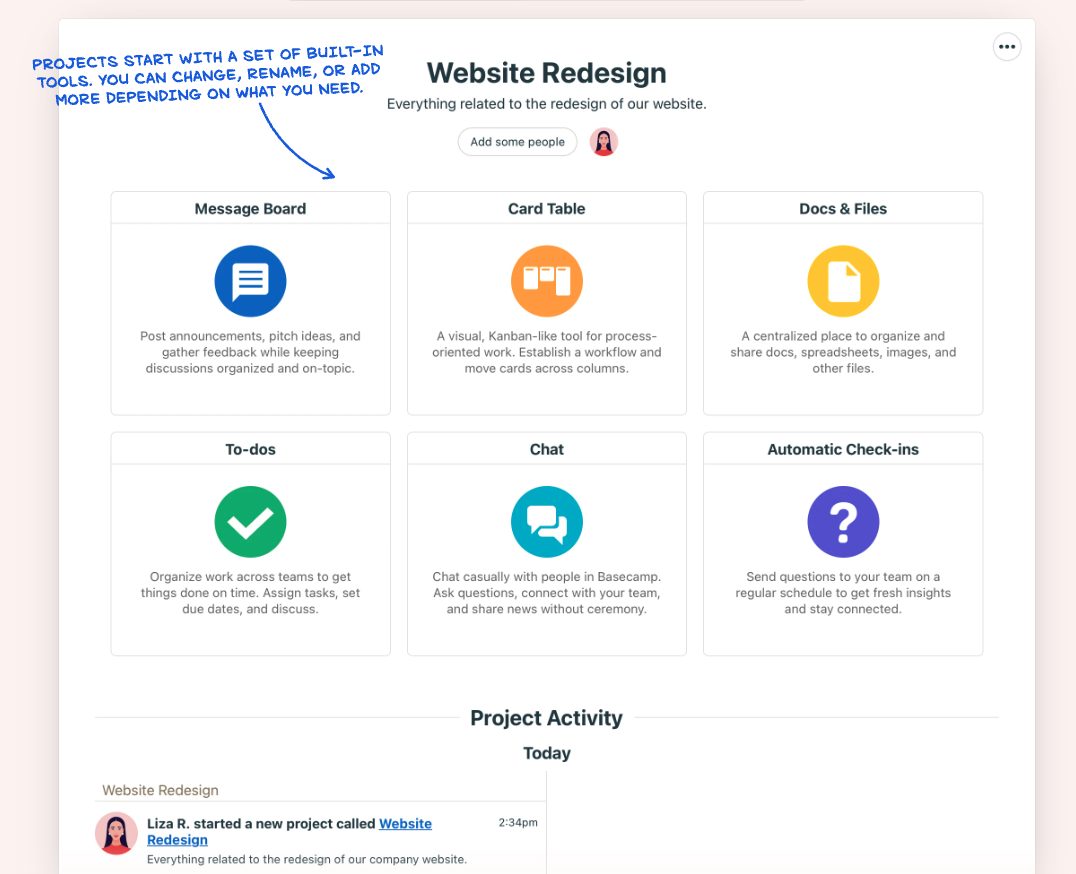
\includegraphics[width=0.8\textwidth]{pics/basecamp-project-overview.png}
    \caption{Basecamp Projekt}
    \cite{basecamp_project}
    \label{fig:mesh1}
\end{figure}

Es gibt ein sogenanntes \textbf{Message Board}, in welchen Ankündigungen oder ähnliche wichtige Nachrichten gespeichert werden können. Des weiteren gibt es einen Card Table, welcher ein Kanban Board beinhaltet, welches einen agilen Projektverlauf unterstützt. Dokumente oder wichtige Datein können im Unterpunkt \textbf{Docs und Files} abgespeichert werden. Für To-dos oder auch für den allgemeinen Chat gibt es ebenfalls Unterseiten. Und zuletzt gibt es die Möglichkeit automatische Check-ins zu machen um aktiv mit den anderen Teammitgliedern vernetzt und am laufenden Stand zu sein.

Wir haben dabei hauptsächlich die To-dos und die Chat-Funktion verwendet. Erwähnenswert ist auch, dass die Kommunikation ausschließlich über Basecamp stattgefunden hat und die Arbeit damit im Allgemeinen gut funktioniert hat.

\begin{spacing}{1}
\chapter{Umfeldanalyse}
\end{spacing}
\lipsum[4] Citing \cite{InfH} properly.

Was ist eine \gls{guid}?
Eine \gls{guid} kollidiert nicht gerne.

Kabellose Technologien sind in abgelegenen Gebieten wichtig \cite{APCW2006}.


\begin{spacing}{1}
\chapter{Technologien}\label{chapter:tech}
\end{spacing}
\section{Foo}
\setauthor{Stefan Schwammal}
\lipsum[5-12]

\section{Bar}
\setauthor{Susi Schwammal}
\lipsum[12-18]

\subsection{Deeper}
Nicht mehr im Inhaltsverzeichnis.

\subsubsection{Deepest}
Vermeide mich.

\begin{spacing}{1}
\chapter{Umsetzung}\label{chapter:implementation}
\end{spacing}
Siehe tolle Daten in Tab. \ref{tab:impl:data}.

\begin{table}
    \centering
    \begin{tabular}{|lcc|}
    \hline
              & \textbf{Regular Customers} & \textbf{Random Customers} \\ \hline
    Age       & 20-40                      & \textgreater{}60          \\ \hline
    Education & university                 & high school               \\ \hline
    \end{tabular}
    \caption{Ein paar tabellarische Daten}
    \label{tab:impl:data}
\end{table}

\begin{figure}
    \centering
    
\includegraphics[scale=0.5]{pics/knuthi.jpg}
    \caption{Don Knuth -- CS Allfather}
    \label{fig:impl:knuth}
\end{figure}

Siehe und staune in Abb. \ref{fig:impl:knuth}.
\lipsum[6-9]
Dann betrachte den Code in Listing \ref{lst:impl:foo}.

\begin{lstlisting}[language=Python,caption=Some code,label=lst:impl:foo]
# Program to find the sum of all numbers stored in a list (the not-Pythonic-way)

# List of numbers
numbers = [6, 5, 3, 8, 4, 2, 5, 4, 11]

# variable to store the sum
sum = 0

# iterate over the list
for val in numbers:
    sum = sum+val

print("The sum is", sum)
\end{lstlisting}

\begin{spacing}{1}
\chapter{Zusammenfassung}
\end{spacing}
Aufzählungen:

\begin{compactitem}
    \item Itemize Level 1
    \begin{compactitem}
        \item Itemize Level 2
        \begin{compactitem}
            \item Itemize Level 3 (vermeiden)
        \end{compactitem}
    \end{compactitem}
\end{compactitem}

\begin{compactenum}
    \item Enumerate Level 1
    \begin{compactenum}
        \item Enumerate Level 2
        \begin{compactenum}
            \item Enumerate Level 3 (vermeiden)
        \end{compactenum}
    \end{compactenum}
\end{compactenum}

\begin{compactdesc}
    \item[Desc] Level 1
    \begin{compactdesc}
        \item[Desc] Level 2 (vermeiden)
        \begin{compactdesc}
            \item[Desc] Level 3 (vermeiden)
        \end{compactdesc}
    \end{compactdesc}
\end{compactdesc}

\newpage
\pagenumbering{Roman}
\setcounter{page}{\value{RPages}}
\newacronym{guid}{GUID}{Globally Unique Identifier}
\newacronym{jit}{JIT}{Just In Time Compiler}
\newacronym{nfc}{NFC}{Near Field Communication}
\newacronym{rfid}{RFID}{Radio Frequency Identification}

% Usage:
% \gls{label} lowercase in text
% \Gls{label} Uppercase in text
% \newacronym{label}{abbrev}{full}
% \newglossaryentry{label}{settings}



%\setlength{\glsdescwidth}{0.8\linewidth}
\glsnogroupskiptrue
\printglossary[title=Glossar,toctitle=Glossar] %,style=long]
\spacing{1}{
%\bibliographystyle{IEEEtran}
\bibliographystyle{ieeetrande}
\bibliography{bib}
}
\listoffigures
\listoftables
\lstlistoflistings
\appendix
\addchap{Anhang}
\input{./sections/appendix}
\end{document}

